\section{Results}
\subsection{The DeepPBS Framework}
The DeepPBS framework is illustrated in \hyperref[fig:pdna1]{Fig. 2.2}. Input to DeepPBS (\hyperref[fig:pdna1]{Fig. 2.2a}) is composed of one protein-DNA complex structure, with one or more protein chains bound to a DNA double helix. Potential sources for such structures include experimental data (for example, PDB\citep{berman2000protein}), molecular simulation snapshots or designed complexes. DeepPBS processes the structure as a bipartite graph with distinct spatial graph representations for protein and DNA components. The protein graph is an atom-based graph, with heavy atoms as vertices. Several features are computed on these vertices (\hyperref[fig:pdna1]{Fig. 2.2b}). Further information on protein representation and feature computation is available in Methods. We represent DNA as a symmetrized helix (sym-helix), as detailed in Methods. This representation removes any sequence identity that the DNA possesses, while preserving the shape of the double helix \citep{rohs2009role}. Optionally, DNA sequence information can be reintroduced as a feature on the sym-helix points.
\par
DeepPBS performs a series of spatial graph convolutions on the protein graph to aggregate atomic neighborhood information (\hyperref[fig:pdna1]{Fig. 2.2d}). The next crucial component of DeepPBS consists of a set of bipartite geometric convolutions applied from the protein graph to the sym-helix (\hyperref[fig:pdna1]{Fig. 2.2d}). Specific chemical interactions (for example, hydrogen bonds) depend on both location and orientation \citep{Helene1977}. DeepPBS learns how the geometric orientation of the sym-helix points is associated with the orientations and chemistry of neighboring protein residues. Four distinct bipartite convolutions are employed for the sym-helix points, corresponding to the major groove, the minor groove and the phosphate and sugar moieties. Major and minor groove convolutions are referred to as ‘groove readout’. This term was chosen over the term ‘base readout’ due to the removal of base identity in the sym-helix. Phosphate and sugar moiety convolutions, combined with DNA shape information, form the ‘shape readout’ (\hyperref[fig:pdna1]{Fig. 2.2e}). The ‘groove readout’ and ‘shape readout’ factors collaboratively determine binding specificity to varying extents for different protein families. At this point, the sym-helix representation enables a straightforward flattening of aggregated features on the three-dimensional sym-helix to the one-dimensional (1D) base pair-level features. By adding DNA shape information and implementing 1D convolutional neural network and prediction layers (\hyperref[fig:pdna1]{Fig. 2.2e}), DeepPBS ultimately predicts binding specificity (\hyperref[fig:pdna1]{Fig. 2.2f}). Further architectural details are described in Supplementary Section 5.
\par
Lack of an existing published standard dataset for predicting binding specificity across protein families from protein-DNA complex structure data made it necessary for us to build a dataset for cross-validation and benchmarking. Details of this process can be found in Methods.

\begin{center}
    \begin{figure}
    \makebox[\textwidth]{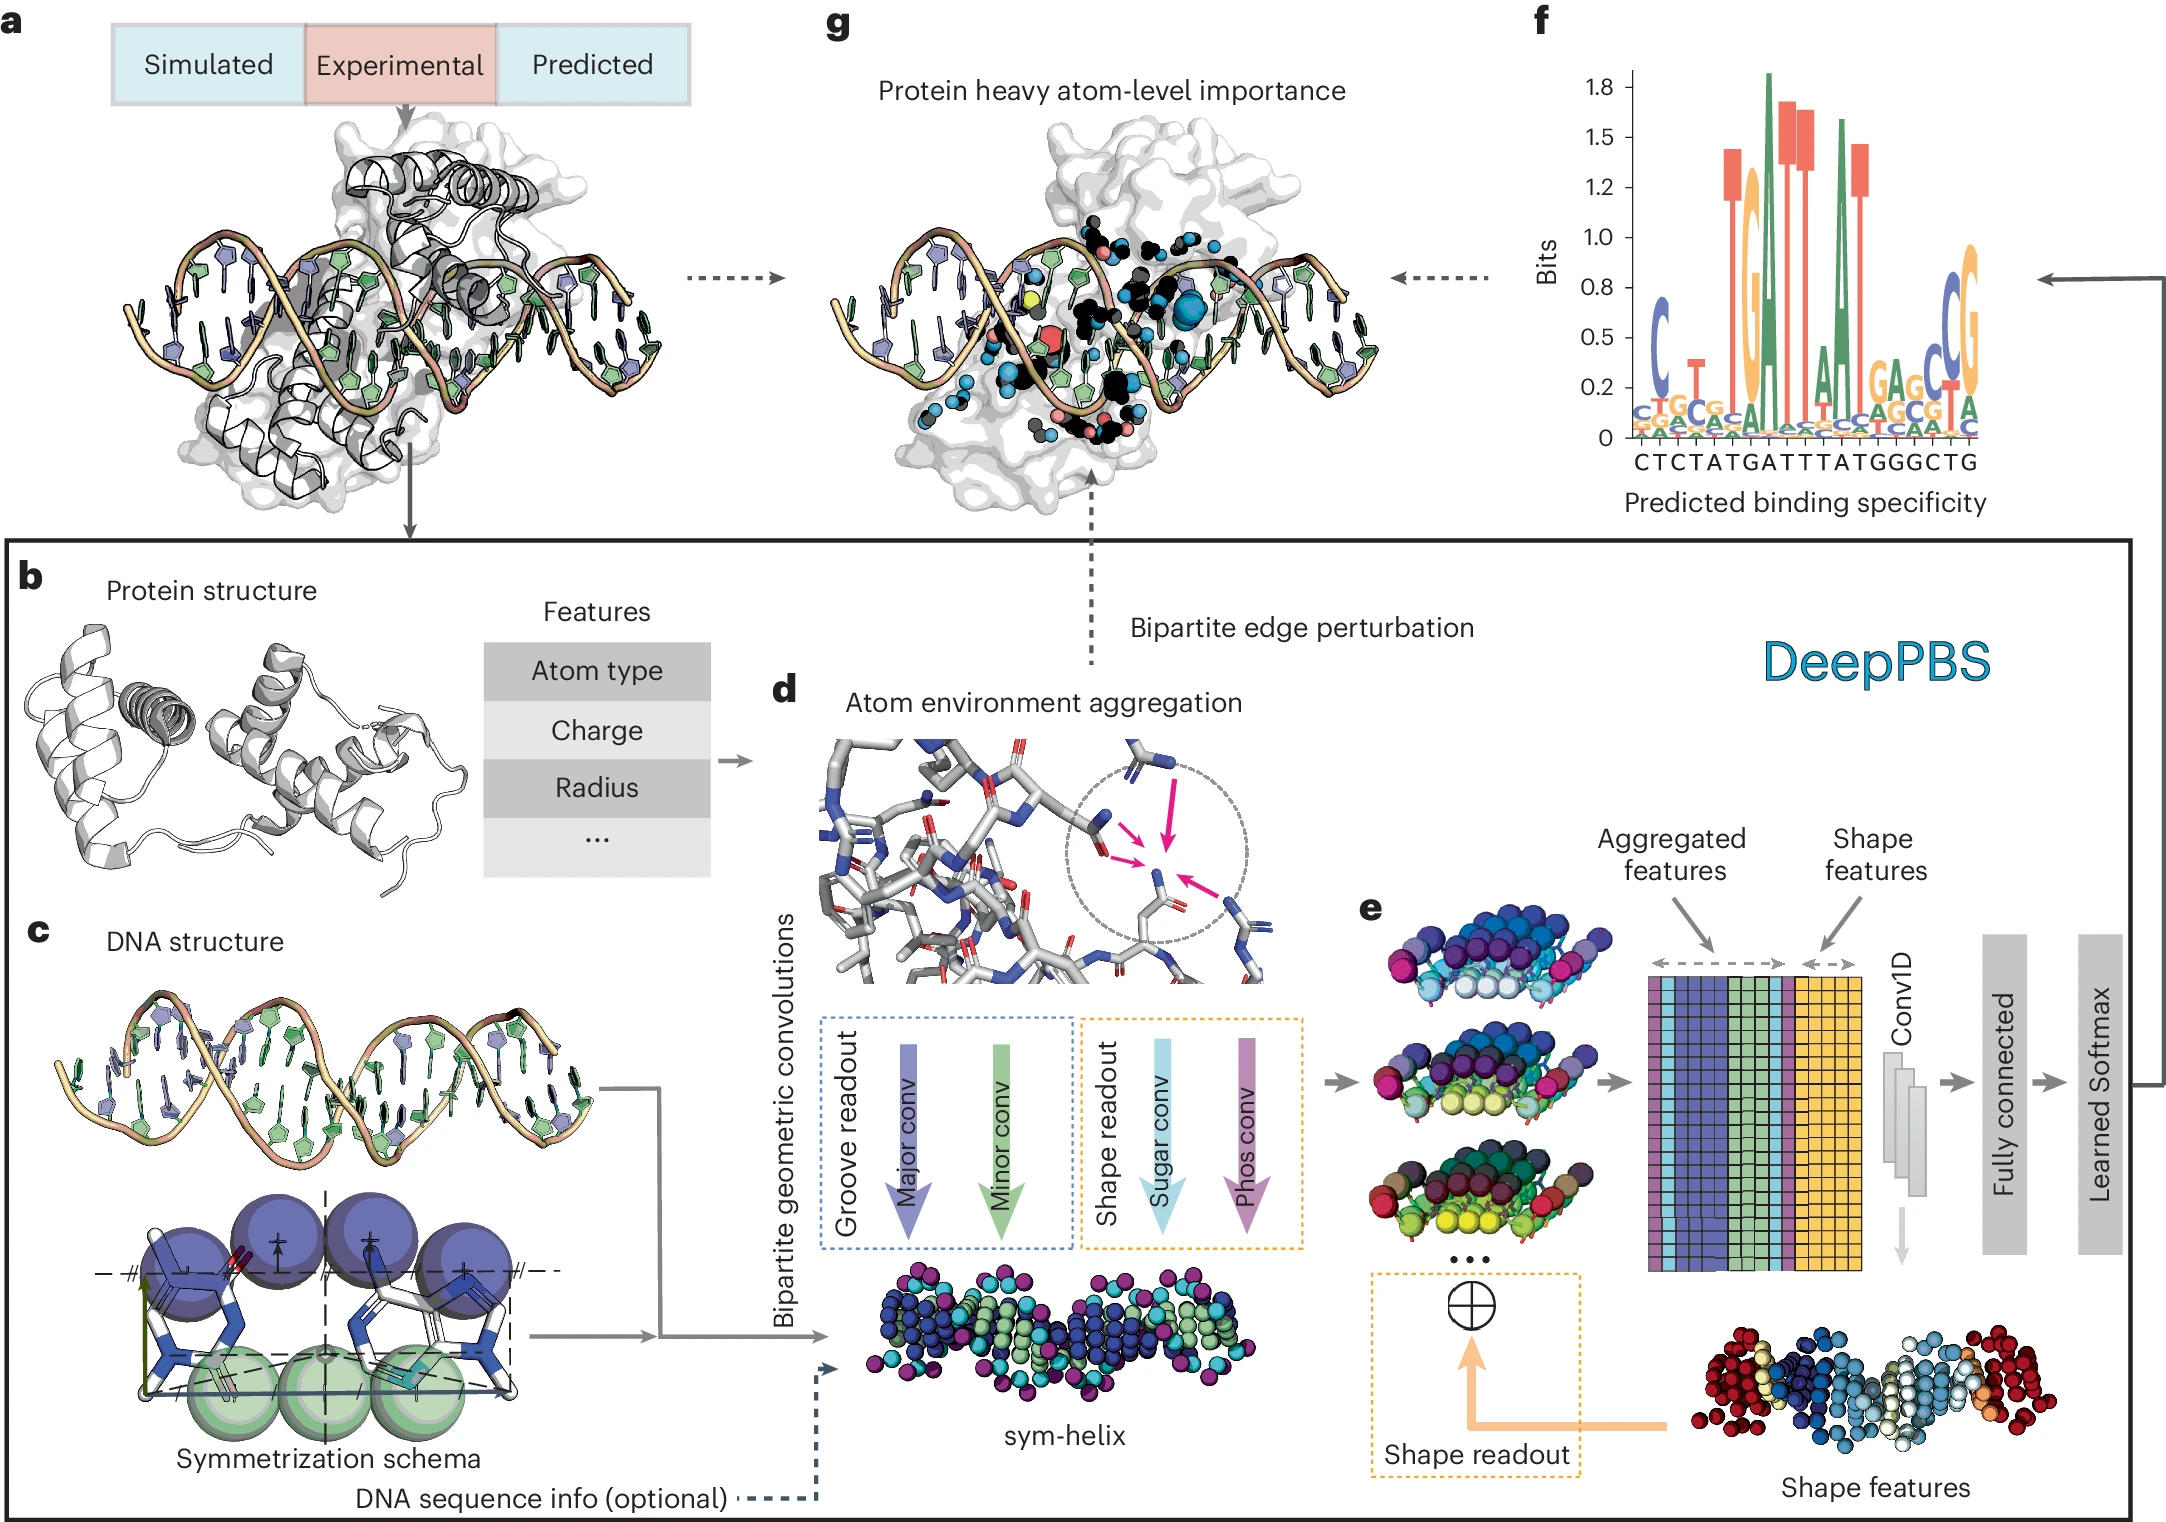
\includegraphics[width=0.8\paperwidth]{./pdnafigs/fig1.png}}
 % archetecture.png: 1149x508 px, 72dpi, 40.53x17.92 cm, bb=0 0 1149 508
        \caption[Schematic illustration of the DeepPBS framework]{\textbf{| Schematic illustration of the DeepPBS framework.} ({\bf a}) DeepPBS input
(PDB ID 2R5Y in this example) and possible input sources. ({\bf b}) Protein structure (heavy atom graph, with features computed for each vertex). ({\bf c}) Symmetrization schema in base-pair frame applied to DNA structure, resulting in a sym-helix. ({\bf d}) Spatial graph convolution on the protein graph for atom environment aggregation, followed by bipartite geometric convolutions from protein graph vertices to sym-helix points (shown as spheres with specific colors for major groove, minor groove, phosphate and sugar). ({\bf e}) Three-dimensional sym-helix is flattened with aggregated information (concatenated with computed shape features) into a 1D representation, followed by 1D convolutions and regression onto base pair probabilities. ({\bf f}) DeepPBS outputs binding specificity. ({\bf g}) Effect of perturbing bipartite edges involved in d can be measured in terms of changes in the output, providing an effective measure of interpretability. Phos, phosphate; conv, convolutions.}
  \label{fig:pdna1}
\end{figure}
\end{center}

\subsection{DeepPBS performance for experimentally determined structures}
The DeepPBS ensemble (Methods) was employed to evaluate model performance against a benchmark set, as outlined in Supplementary Section 1. The DeepPBS architecture allows models to be trained on two mechanisms: ‘groove readout’, which does not involve backbone convolutions and excludes shape information, and ‘shape readout’, which does not involve groove convolutions (\hyperref[fig:pdna1]{Fig. 2.2d,e}). Benchmark performances of DeepPBS (which performs both ‘groove readout’ and ‘shape readout’ modes combined) and these two variations are shown in \hyperref[fig:pdna2]{Fig. 2.3a}. The ‘groove readout’ version does better than the ‘shape readout’ version in terms of median performance, while the DeepPBS model improves upon either component in isolation (two-sided t-test P value <0.01; \hyperref[fig:pdna2]{Fig. 2.3a}). 
\par
The dataset was constructed using experimentally determined structures; thus, the co-crystal structure-derived DNA sequence typically serves as a reasonable example of a bound sequence. As expected, integrating sequence information into the sym-helix points (‘DeepPBS with DNA SeqInfo’) enhanced performance (\hyperref[fig:pdna2]{Fig. 2.3a}), significantly closing the gap toward the inherent performance limit in the dataset. The inherent performance limit originates from the fact that for the same protein the binding specificity data presented by two databases \citep{Jaime2022, kulakovskiy2018hocomoco} used to create the dataset may disagree to some extent (Supplementary \hyperref[fig:pdnaS1]{Fig. S1c}). We computed the distribution of disagreement across all unique PWMs appearing in both databases (Supplementary Section 1). However, from both interpretability and design perspectives, particularly when the bound DNA sequence may not be representative, the ‘DeepPBS’ model is optimal due to its low sensitivity to the DNA sequence in the structure. This fact is evidenced by comparing performances of the ‘DeepPBS’ and ‘DeepPBS with DNA SeqInfo’ models in the context of the PWM-co-crystal-derived DNA alignment score (Supplementary Section 1). Compared with the line fit to the variation with DNA sequence information (slope $-0.44$ for root mean squared error (RMSE), slope $-0.62$ for mean absolute error (MAE); Supplementary \hyperref[fig:pdnaS11]{Fig. S11}), the slope of the line fit to the DeepPBS predictions was closer to zero (\hyperref[fig:pdna2]{Fig. 2.3b} and Supplementary \hyperref[fig:pdnaS11]{Fig. S11}).
\par
As an example, we show the DeepPBS ensemble prediction for the NF-$\kappa$B biological assembly from the benchmark dataset. Although the co-crystal structure-derived DNA sequence was not of the highest binding affinity, as indicated by experimental data from HOCOMOCO \citep{kulakovskiy2018hocomoco}, our prediction circumvented this issue, predicting a binding specificity that was more closely aligned with the experimental data (Supplementary \hyperref[fig:pdnaS5]{Fig. S5d}). Similar trends (Supplementary \hyperref[fig:pdnaS5]{Fig. S5a-c}) can be observed from cross-validation predictions by individual DeepPBS models (Methods). We also included example DeepPBS ensemble predictions (Supplementary \hyperref[fig:pdnaS7]{Fig. S7}) for structures in the PDB that correspond to specific interactions but do not have a PWM in the two binding specificity databases considered (Methods). In addition, example DeepPBS ensemble predictions (Supplementary \hyperref[fig:pdnaS8]{Fig. S8}) for structures of nonspecific protein-DNA binding (for example, SSO7D-DNA interaction \citep{Agback1998}) present in the PDB are presented. These predictions have notably lower information content compared with those in Supplementary \hyperref[fig:pdnaS7]{Fig. S7}.

\subsection{DeepPBS captures patterns of family-specific binding modes}
Abundances of different protein families in the benchmark set are described in \hyperref[fig:pdna2]{Fig. 2.3c} (Supplementary \hyperref[fig:pdnaS5]{Fig. S5b} for cross-validation set). Family annotations were obtained from the Database of Protein Families (PFAM) \citep{Mistry2021}. The dataset encompasses a wide range of DNA-binding protein families. Performance of DeepPBS for various protein families provides several key insights. DeepPBS showed reasonable generalizability across protein families, performing well even for families with relatively fewer structures (\hyperref[fig:pdna2]{Fig. 2.3d} and Supplementary \hyperref[fig:pdnaS5]{Fig. S5c}), such as heat shock factor proteins. This observation suggests that the model is learning the underlying mechanisms of protein-DNA binding rather than overfitting on family-specific patterns.
\par
Further validation is provided by comparing performances of the DeepPBS ‘groove readout’ and ‘shape readout’ models (\hyperref[fig:pdna2]{Fig. 2.3d} and Supplementary \hyperref[fig:pdnaS5]{Fig. S5c}). For families like zf-C$_2$H$_2$, zf-C$_4$ the ‘shape readout’ model did not perform as well as the ‘groove readout’ model. This result aligns with the common understanding of the binding mechanism of these families. For example, zf-C$_2$H$_2$ uses zinc finger motifs to scan DNA for suitable base interactions, with minimal DNA bending or conformational change \citep{Persikov2011}. This binding mode makes the zf-C$_2$H$_2$ family a popular target of protein sequence-based binding specificity prediction and design \citep{Persikov2014, persikov2009predicting, Sofia2022, Yanover2011, Ichikawa2023}. Conversely, families like interferon-regulatory factor (IRF) proteins (\hyperref[fig:pdna2]{Fig. 2.3d} and Supplementary \hyperref[fig:pdnaS5]{Fig. S5c}) and T-box proteins (Supplementary Fig. 5c) showed higher performances for the ‘shape readout’ model, consistent with their known binding mechanisms that involve significant conformational changes\citep{Stirnimann2010, Escalante1998}. For families such as homeodomain (HD) and forkhead (\hyperref[fig:pdna2]{Fig. 2.3d} and Supplementary \hyperref[fig:pdnaS5]{Fig. S5c}), the DeepPBS model outperformed both the ‘groove readout’ and ‘shape readout’ components. This result suggests that the network captures complex higher-order relationships of these components. 

\begin{center}
    \begin{figure}
    \makebox[\textwidth]{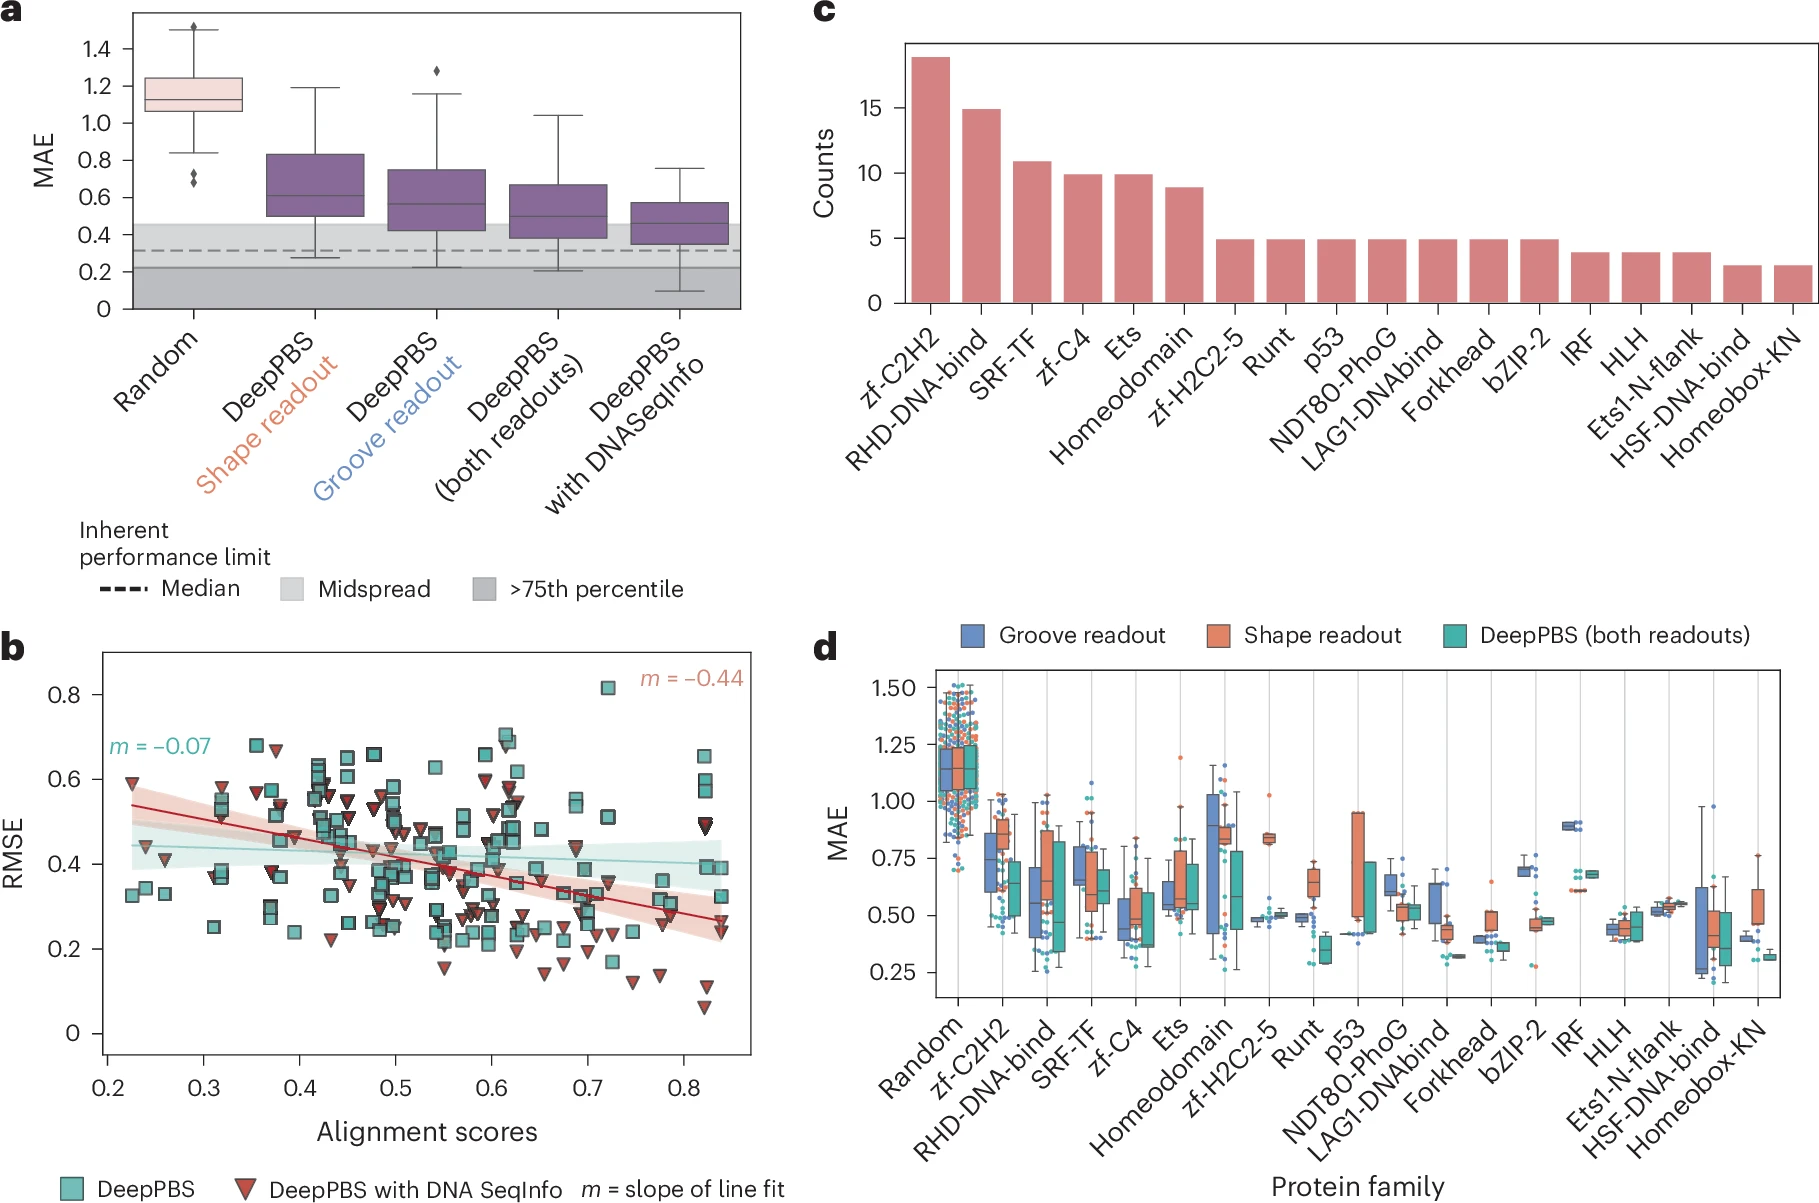
\includegraphics[width=0.8\paperwidth]{./pdnafigs/fig2.png}}
 % archetecture.png: 1149x508 px, 72dpi, 40.53x17.92 cm, bb=0 0 1149 508
        \caption[Performance of DeepPBS for predicting binding specificity across
protein families for experimentally determined structures.]{\textbf{Performance of DeepPBS for predicting binding specificity across
protein families for experimentally determined structures.} ({\bf a}) Prediction performances of DeepPBS along with ‘groove readout’, ‘shape readout’ and ‘with DNA SeqInfo’ variations, on benchmark set (biological assemblies corresponding to $n$ = 130 protein chains (for each box plot); Supplementary Section 1). MAE, mean absolute error; RMSE, root mean squared error. ({\bf b}) Performances of DeepPBS and ‘with DNA SeqInfo’ models in context of PWM–co-crystal-derived DNA alignment score (Supplementary Section 2). The shaded regions indicate
the 95\% confidence interval for the corresponding linear fit. The MAE equivalent of this plot is available as Supplementary Fig. 12, showing similar trends. ({\bf c}) Abundances of various protein families (as appearing in PFAM annotations) in constructed benchmark set (counts $>$3). ({\bf d}) Performances of DeepPBS, groove readout and shape readout models across various protein families (counts $>$3) (biological assemblies corresponding to n protein chains (for each family), where $n$ is as described in ({\bf c}), total unique $n$ = 130). All benchmark predictions are made by an ensemble average of five models trained via cross-validation. Cross-validation performances of individual trained models are shown in Supplementary \hyperref[fig:pdnaS5]{Fig. S5c}. For the box plots in ({\bf a}) and ({\bf d}), the lower limit represents the lower quartile, the middle line represents the median and the upper limit represents the upper quartile.}
  \label{fig:pdna2}
\end{figure}
\end{center}

\subsection{Application to in silico-predicted protein–DNA complexes}
The DeepPBS framework is not limited to experimental structures. Recent advances in scalable structural prediction approaches, driven by artificial intelligence \citep{Jumper2021, Baek2021}, offer unprecedented potential. Specifically, models like RFNA \citep{baek2024na} and MELD-DNA \citep{Esmaeeli2023} can be used to predict the structures of protein-DNA complexes from sequence. Such prediction algorithms have paved the way for DeepPBS to be applicable to proteins that lack experimental DNA-bound structure data.
\par
We suggest one potential approach for working with predictive structures in DeepPBS. First, we make an initial guess for the DNA (IG DNA) sequence bound to each protein of interest based on the corresponding protein family. Then, we use RFNA to predict the protein-DNA complex structure, followed by DeepPBS to predict binding specificity. We demonstrate this process (\hyperref[fig:pdna3]{Fig. 2.4a-c}) for three proteins classified as basic helix-loop-helix (bHLH) in JASPAR \citep{Jaime2022}. In all three cases, the PDB lacked experimental protein-DNA complex structures. The IG DNA (Supplementary Section 8) has an enhancer box motif (‘CACGTG’) in the center, which is known \citep{demartin2021} to be a bHLH family target. The first example (UniProt Q4H376; \hyperref[fig:pdna3]{Fig. 2.4a}) is a Max homodimer, for which DeepPBS predicted a specificity closely mirroring that of the IG DNA. The second example (TCF21 dimer, O43680) was more complicated; the central ‘CACGTG’ motif in the IG DNA was erroneously assumed, yet DeepPBS successfully predicted the correct motif as ‘CATATG’ (\hyperref[fig:pdna3]{Fig. 2.4b}). The third example (\hyperref[fig:pdna3]{Fig. 2.4c}, protein OJ1581$\_$H09.2, Q6H878) does not conform to any enhancer box motif. Nevertheless, DeepPBS predicted a binding specificity closely mirroring the experimental data (\hyperref[fig:pdna3]{Fig. 2.4c}).
\par
We ran the DeepPBS pipeline for full-length UniProt protein sequences, each with a unique JASPAR entry and no experimental structure for the complex, across three different families (Supplementary Section 8): bZIP, bHLH and HD families. DeepPBS predictions based on RFNA-predicted structures exhibited an improved MAE (that is, closer to experimental data) compared with the IG DNA baseline (\hyperref[fig:pdna3]{Fig. 2.4d}). An application of DeepPBS to a MELD-DNA-predicted complex of the mouse CREB1 protein is demonstrated in Supplementary \hyperref[fig:pdnaS9]{Fig. S9b}. Thus, DeepPBS can take predicted structures from suboptimal DNA sequences and predict binding specificity close to experimental data.
\par
We next explored whether DeepPBS prediction could be used as feedback (in a loop) to enhance modeling of the protein complex (and, subsequently, improve DeepPBS prediction). We demonstrated this process for the human TGIF2LY protein (UniProt ID Q8IUE0, unstructured region trimmed; Supplementary Section 8) in \hyperref[fig:pdna3]{Fig. 2.4e}. In round 1, we applied RFNA to this protein sequence alongside the IG DNA sequence for the HD family and then used the predicted complexes as input for DeepPBS. For IG DNA position T15 (\hyperref[fig:pdna3]{Fig. 2.4e}, round 1), DeepPBS predicted a strong preference for G. In the round 1 RFNA output, Arg57 and T15 were involved in one hydrogen bond (H-bond) and one van der Waals interaction. These interactions are theoretically weaker than the possible bidentate H-bonds between a G and Arg57. In round 2, we altered the RFNA input by taking the argmax (the most preferred sequence) from the DeepPBS output (\hyperref[fig:pdna3]{Fig. 2.4e}, round 2). The subsequently folded structure reflected a more robust bidentate H-bond interaction between G15 and Arg57, with the DeepPBS prediction more closely aligning with the experimental data (note positions (round 2) A18, G19 and T14, corresponding to positions 4-6 in MA1572.1; \hyperref[fig:pdna3]{Fig. 2.4e}).
\par
We repeated this DeepPBS prediction process for a total of seven rounds, for the set of HD monomer sequences (Supplementary Section 8). The RFNA-predicted confidence metric (predicted local distance difference test (pLDDT), LDDT \citep{Mariani2013} reflects similarity between the predicted and reference structure for a complex; Supplementary Section 8) improved over these rounds (\hyperref[fig:pdna3]{Fig. 2.4f}). To independently evaluate structure quality, we calculated the molecular mechanics and Poisson-Boltzmann surface area \citep{Genheden2015} binding energy (Supplementary Section 8). From round 1 to round 3+, the number of stable structures (binding energy $kJ/mol$) increased (Supplementary \hyperref[fig:pdnaS9]{Fig. S9c}), while their binding energy distributions shifted toward lower values (Supplementary \hyperref[fig:pdnaS9]{Fig. S9c}). DeepPBS performance improved across the five rounds (Supplementary \hyperref[fig:pdnaS9]{Fig. S9a}). We also refolded the benchmark set datapoints via RFNA (Supplementary Section 8) and compared (for the full processable set ($n=98$) and a high-confidence set, pLDDT $>$0.9, $n=31$) the performances with the equivalent performance obtained for the experimental structures (\hyperref[fig:pdna3]{Fig. 2.4g}). There is a drop in performance. We can expect that it will improve when future models for structure prediction become available.
\par
The DeepPBS approach for predicting binding specificity fundamentally differs from that of existing methods, which predict binding specificity solely on the basis of protein sequence information. As a result, comparisons with existing family-specific methods that operate exclusively on protein sequence are unfeasible. However, in conjunction with a complex structure prediction method, we can start from protein sequence information alone and predict binding specificity using DeepPBS. This process can be compared with the recent HD family-specific method, rCLAMPS \citep{Wetzel2022} (Supplementary Section 8). rCLAMPS can predict core 6-mer binding specificities for monomer HD proteins. A comprehensive overview of performances is shown in \hyperref[fig:pdna3]{Fig. 2.4h}. For different significant portions of the data, DeepPBS and rCLAMPS outperformed each other. DeepPBS outperformed rCLAMPS where the pLDDT scores were higher (\hyperref[fig:pdna3]{Fig. 2.4i}). Thus, the DeepPBS pipeline is comparable to rCLAMPS, while having broader applicability across families and biological assemblies as well as not being limited to predicting the DNA core binding region.

\subsection{Assessing protein residue importance at p53-DNA interface}
The DeepPBS architecture permits intentional activation or deactivation of specific edges in the bipartite geometric convolution stage (\hyperref[fig:pdna1]{Fig. 2.2d} and Supplementary \hyperref[fig:pdnaS4]{Fig. S4}). Perturbing a set of edges in this manner will alter the network-predicted result. The mean absolute difference between the original and altered prediction can be used (with proper normalization) as a quantification of the impact of the perturbed set of edges in determining binding specificity (\hyperref[fig:pdna1]{Fig. 2.2g}, Supplementary \hyperref[fig:pdnaS4]{Fig. S4} and Methods).
\begin{center}
    \begin{figure}[H]
    \makebox[\textwidth]{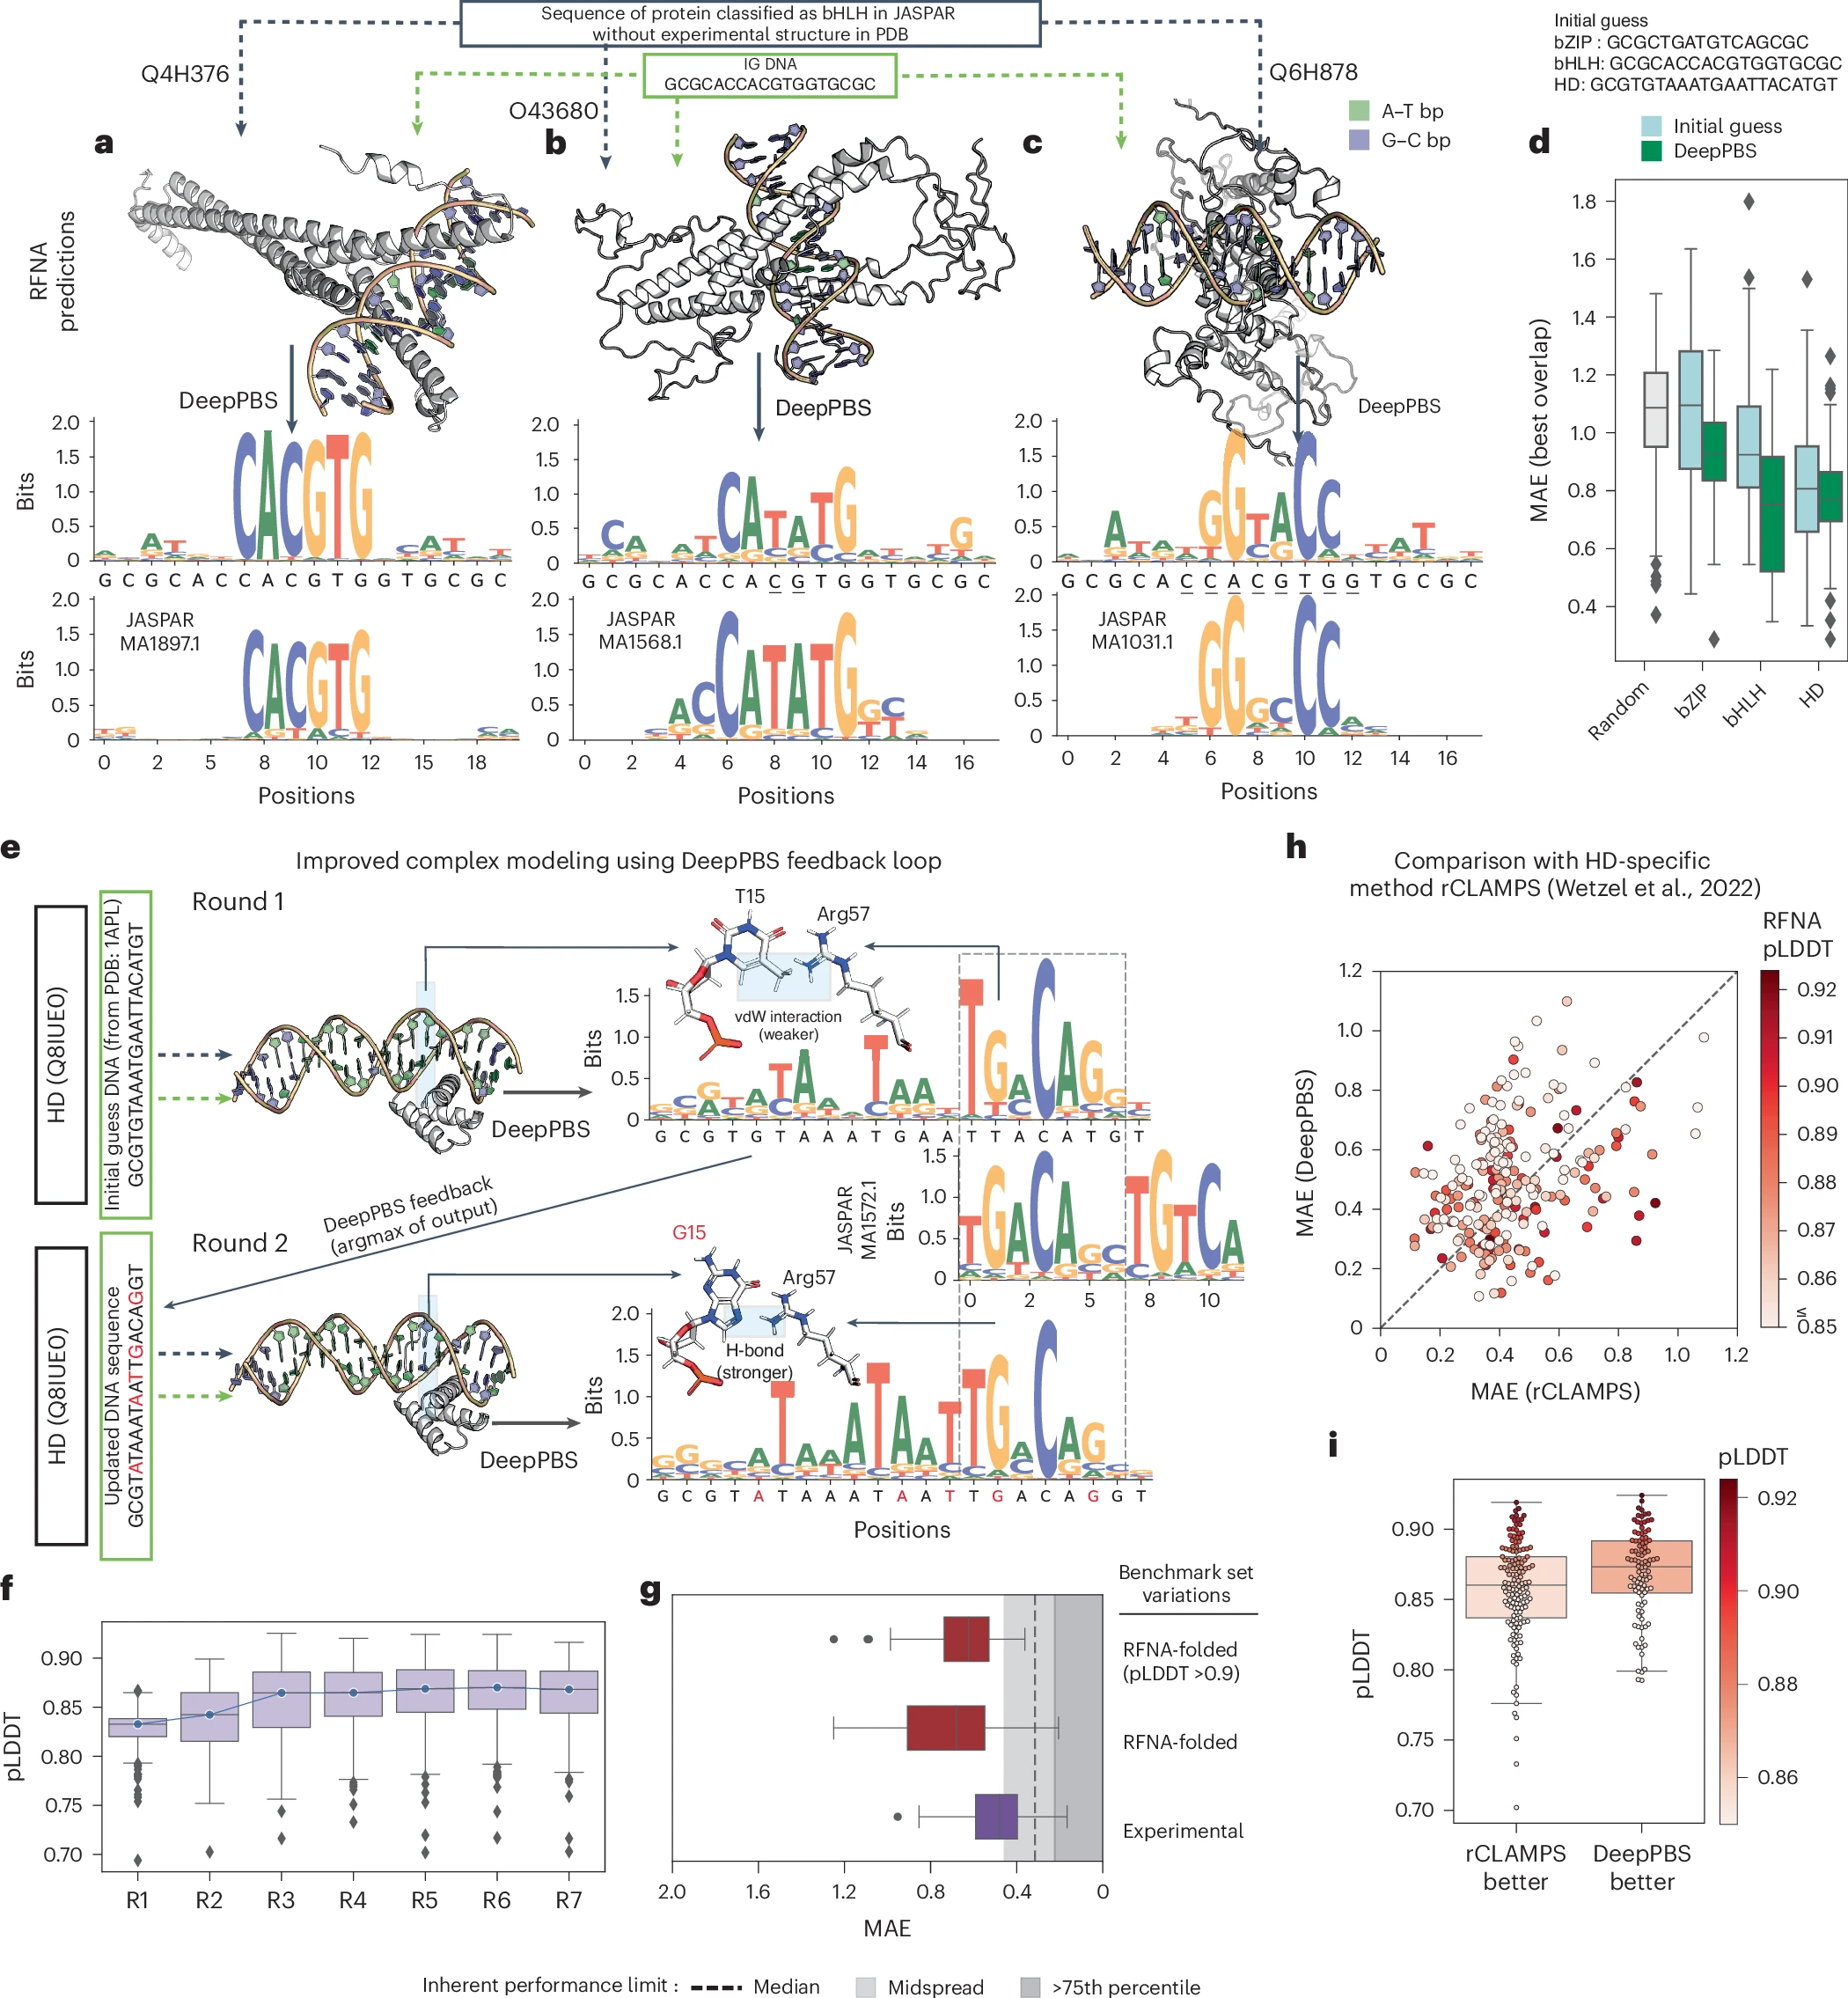
\includegraphics[width=0.8\paperwidth]{./pdnafigs/fig3.png}}
 % archetecture.png: 1149x508 px, 72dpi, 40.53x17.92 cm, bb=0 0 1149 508
        \caption[]{\textbf{Application of DeepPBS on predicted protein–DNA complex structures.} Caption on next page.}
  \label{fig:pdna3}
\end{figure}
\addtocounter{figure}{-1}
\begin{figure} [t!]
  \caption[Application of DeepPBS on predicted protein–DNA complex structures.]{\textbf{Application of DeepPBS on predicted protein–DNA complex structures.} ({\bf a}) Various predictive approaches (for example, RFNA and MELD-DNA) can be used to predict protein–DNA complex structures in the absence of experimental data. DeepPBS can predict binding specificity on the basis of this predicted complex. {\bf a}-{\bf c}, Examples for three full-length bHLH protein sequences: Max homodimer from Ciona intestinalis (a), TCF21 dimer from Homo sapiens ({\bf b}) and OJ1581\_H09.2 dimer from Oryza sativa ({\bf c}). ({\bf d}) Performance of DeepPBS via the same process applied for three different families, bZIP (n = 50 predicted assemblies), bHLH (n = 49 predicted assemblies) and HD (n = 236 predicted assemblies), compared with baselines determined for random (drawn from uniform) and IG DNA sequences. Each protein has a unique JASPAR annotationand lacks an experimental structure for the complex. Structures for protein complexes were predicted by RFNA. Proteins passed the preprocessing criterion of DeepPBS. ({\bf e}) One iteration of DeepPBS feedback, demonstrated for human TGIF2LY protein. vdW, van der Waals. ({\bf f}) RFNA-predicted LDDT 44 score over rounds 1–7 of DeepPBS feedback loop (n = 236 predicted assemblies). ({\bf g}) Comparison of DeepPBS ensemble performance on benchmark set for experimental and RFNA folded structures (for all processable RFNA-folded structures with greater than 500 contact counts (5 Å cutoff) to the DNA helix (n = 98 predicted assemblies) and high confidence (pLDDT $>$0.9) set (n = 31 predicted assemblies)). ({\bf h}) Comparison of DeepPBS predictions against HD family-specific method rCLAMPS, color-coded by pLDDT. Diagonal dashed line represents y = x. ({\bf i}) Distribution of pLDDT for two cases: when DeepPBS outperforms rCLAMPS (below diagonal in h) and vice versa (above diagonal in h) (n = 140 (left) and 96 (right) predicted assemblies). The box colors denote the average pLDDT, using the same colormap as in {\bf h}. For the box plots in {\bf d}, {\bf f}, {\bf g} and {\bf i}, the lower limit represents lower quartile, the center line represents the median and the upper limit represents the upper quartile. The whiskers do not include outliers.}
\end{figure}
\end{center}

\par
We present results for perturbing edge sets for individual protein heavy atoms, which can also be aggregated to compute residue-level importance. As an example, we examined the protein-DNA interface of p53 (PDB ID: 3Q05), a protein crucial for regulating cancer development and cell apoptosis \citep{Joerger2008}. The tumor suppressor p53 binds to DNA as a tetramer with two symmetric protein-DNA interfaces \citep{Kitayner2010, Petty2011}. We show the RI scores (with min-max normalization applied) calculated for heavy atoms within $5\AA$ of the sym-helix (\hyperref[fig:pdna4]{Fig. 2.5a}). Sphere sizes in \hyperref[fig:pdna4]{Fig. 2.5a} denote computed RI scores, with the largest being 1 and smallest 0. Lys120 \citep{Kitayner2006} is involved in both groove readout (H-bond with G) and shape readout-based binding specificity (H-bond with backbone phosphate) (\hyperref[fig:pdna4]{Fig. 2.5b}). The network deems G-Arg280 \citep{Kitayner2006} bidentate H-bonds as another strong driver of binding specificity5 (\hyperref[fig:pdna4]{Fig. 2.5c}). Cys277 confers specificity through its thiol sulfur, accepting an H-bond in the major groove \citep{Kitayner2006} (\hyperref[fig:pdna4]{Fig. 2.5d}). Another important residue according to DeepPBS, Arg248 \citep{Barakat2011}, is present at the minor groove (\hyperref[fig:pdna4]{Fig. 2.5e}). This decision by the model is primarily based on the orientation of arginine relative to the sym-helix, which is devoid of DNA sequence information. Arg248 is attracted through enhanced negative electrostatic potential due to a narrowing of the minor groove where it binds \citep{Kitayner2010}. Among other residues in \hyperref[fig:pdna4]{Fig. 2.5f}, Ser241 is known \citep{Barakat2011} to be important for stabilizing Arg248. Ala276 (known for causing apoptosis upon mutation \citep{Reaz2013}) appears as another driver of specificity. This residue has been shown to be a driver of specificity via van der Waals contacts with the methyl group of T in the major groove\citep{Kitayner2006}. The binding specificity prediction of DeepPBS (\hyperref[fig:pdna4]{Fig. 2.5g}) aligns well with known binding patterns of p53, which follows the form RRRC(A/T)(A/T)GYYY (R denotes purine, and Y denotes pyrimidine). The interactions shown here are deemed \citep{Joerger2008, Vousden2009} as significant drivers of p53 binding.

\subsection{Comparison of residue-level importance with mutagenesis data}
We next asked whether DeepPBS-derived importance scores, which reflect the degree to which an interaction determines output binding specificity, can be considered as reliable and potentially physically significant. Although high-affinity interactions can be nonspecific \citep{Agback1998, Peterson2007}, interactions that contribute to high specificity would be expected to maximize binding affinity across different base pair possibilities. Therefore, the DeepPBS importance scores associated with these interactions should display some correlation with the corresponding binding affinities. We can test this hypothesis experimentally by using alanine scanning mutagenesis data (Supplementary Section 1). Sets of such experimental data have been made available through recent contributions\citep{Ovek2022} in the field. Utilizing these data \citep{Peng2018}, we applied suitable filtering for our context and calculated the log sum aggregated residue level importance scores using DeepPBS (Methods).
\par
A regression plot and Pearson’s correlation coefficient (PCC), as shown in \hyperref[fig:pdna4]{Fig. 2.5h}, illustrate the correspondence between computed values and experimental $\Delta\Delta G$ values for a diverse array of proteins and residues within the protein-DNA interface (Supplementary Table 1). The obtained PCC of 0.60 corroborates our hypothesis. It is noteworthy that the model was not trained to predict these values. These values were only obtained through perturbing the wild-type (WT) structures as input (Supplementary \hyperref[fig:pdna4]{Fig. 2.5} and \hyperref[table:pdna1]{Table 2.1}). These results highlight the potential of DeepPBS as an economical guide for experimentalists who are selecting alanine scanning mutagenesis experiments to conduct at the protein-DNA interface.

\begin{center}
    \begin{figure}
    \makebox[\textwidth]{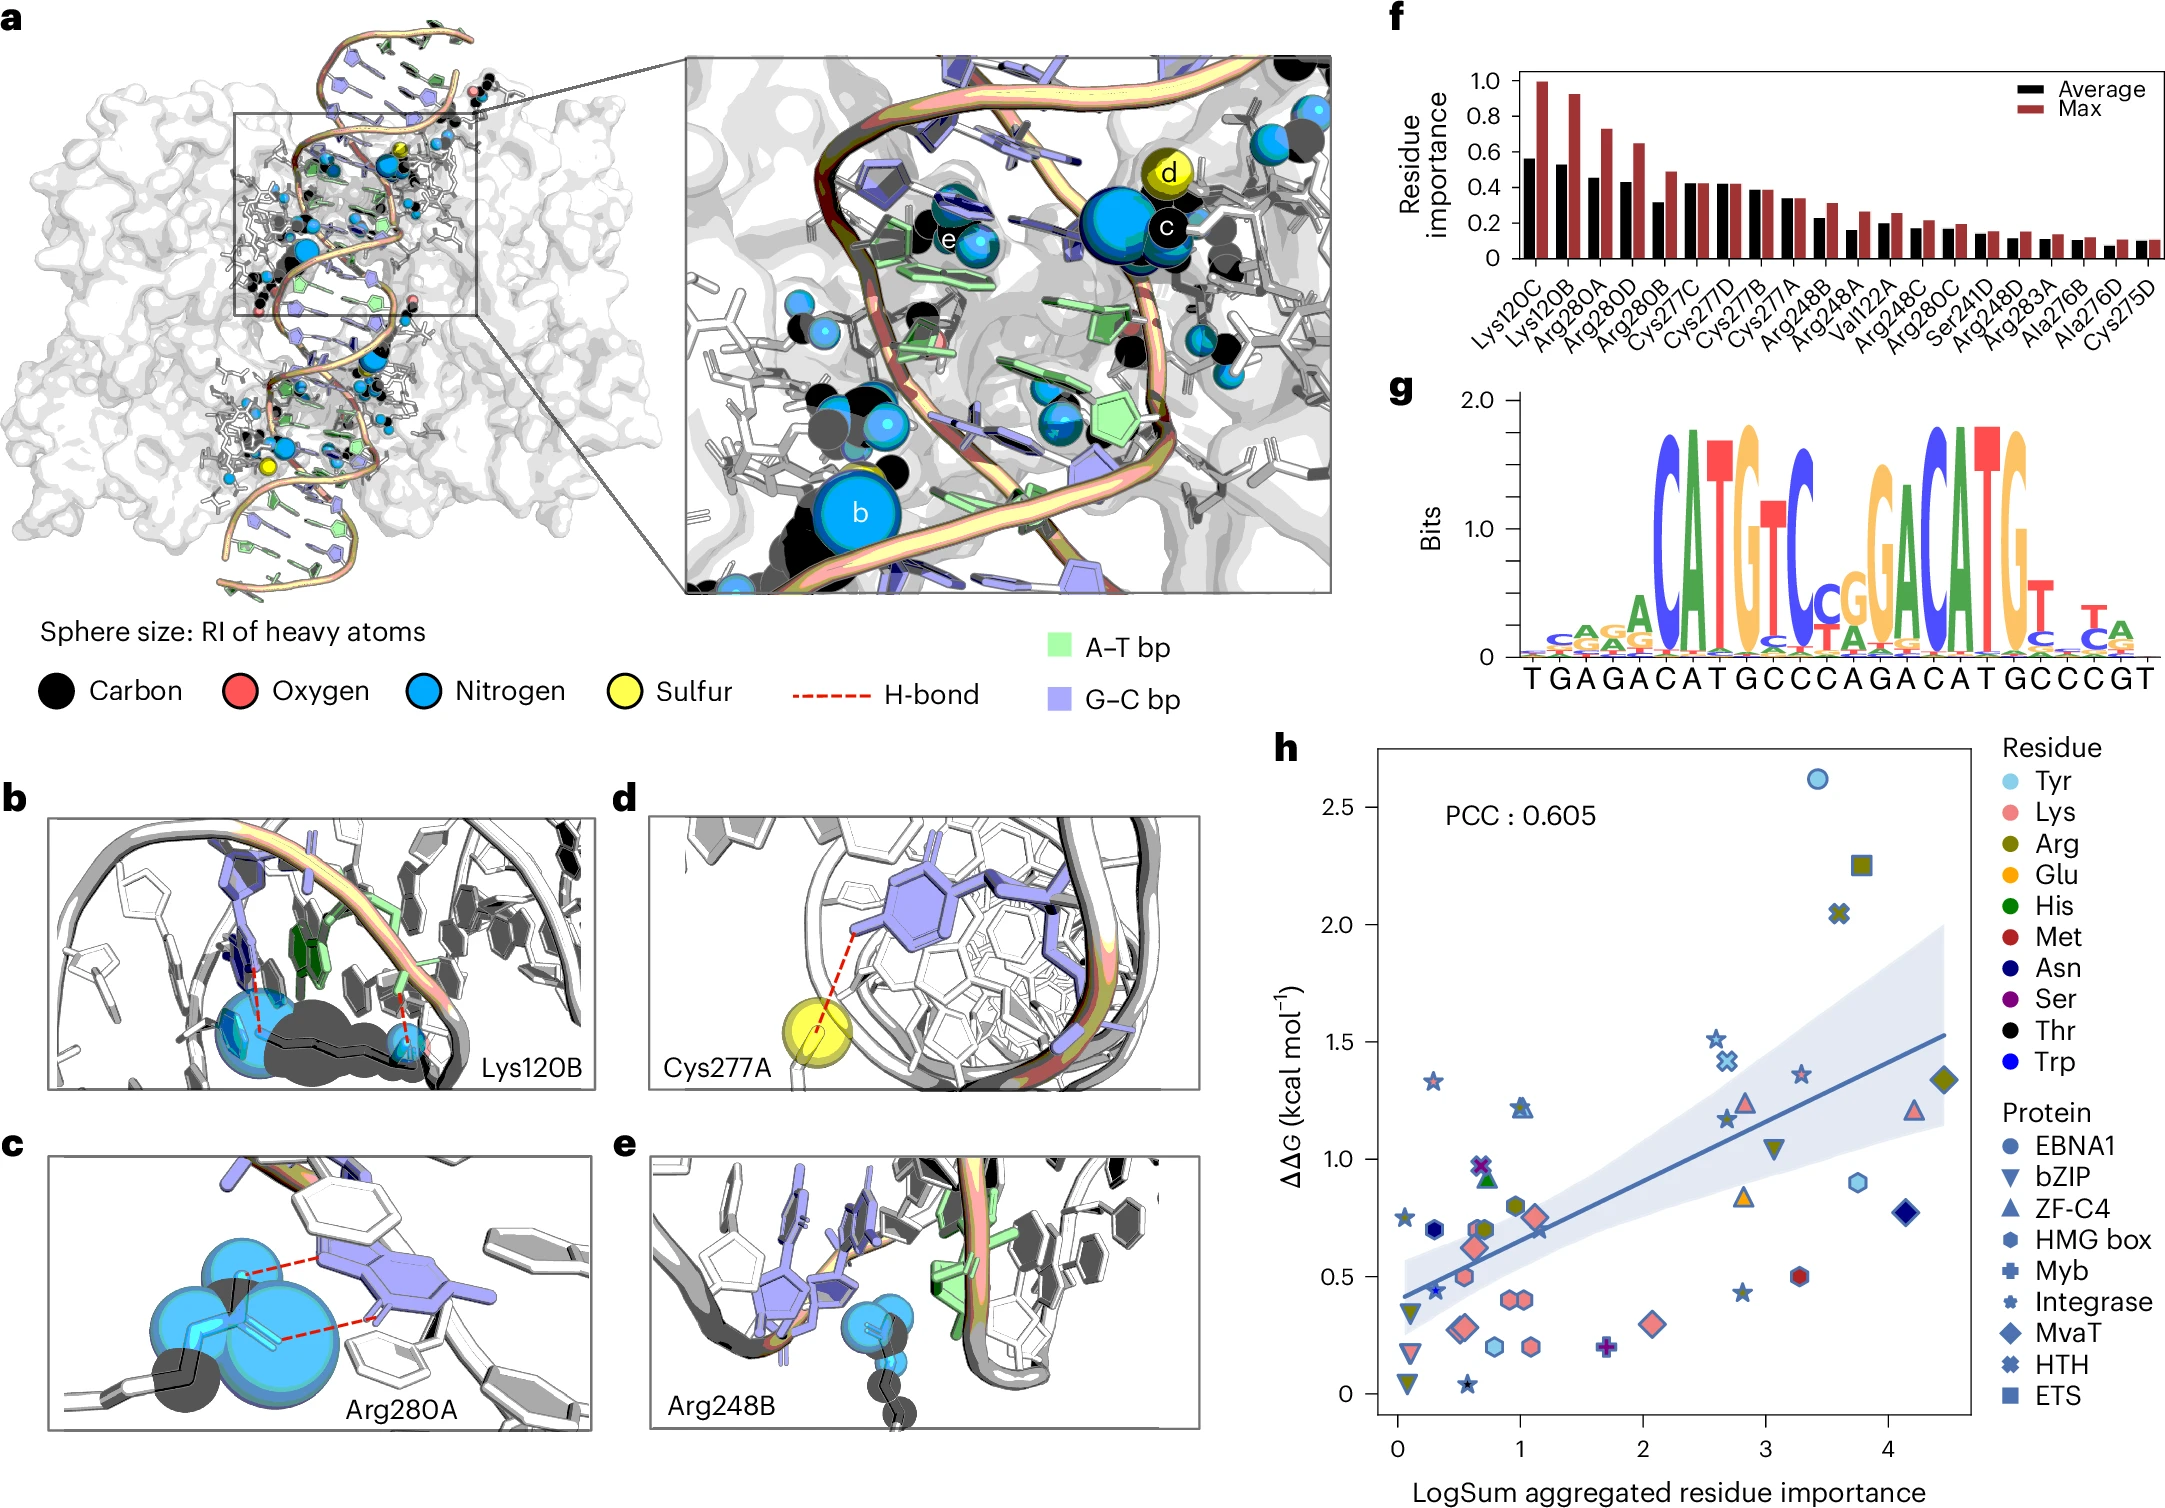
\includegraphics[width=0.8\paperwidth]{./pdnafigs/fig4.png}}
 % archetecture.png: 1149x508 px, 72dpi, 40.53x17.92 cm, bb=0 0 1149 508
        \caption[ Visualization of DeepPBS importance scores in p53–DNA interface as a case study, and experimental validation. ]{\textbf{ Visualization of DeepPBS importance scores in p53–DNA interface as a case study, and experimental validation. } p53 binds to DNA as a tetramer with
two symmetric protein–DNA interfaces 47 (A, B, C and D refer to each monomer; PDB ID: 3Q05). ({\bf a})  Relative importance (RI) score (normalized by maximum across atoms) calculated for heavy atoms (denoted by sphere sizes: largest 1, smallest 0) within 5 $\AA$  of the sym-helix. ({\bf b-e}) , Zoomed-in view of specific interactions by protein–DNA interface residues Lys120B ({\bf b}) , Arg280A ({\bf c}) , Cys277A ({\bf d})  and Arg248B ({\bf e})  with RI scores assigned by DeepPBS. ({\bf f})  Residue importance computed by average and maximum aggregation of heavy atom importance (top 20). ({\bf g})  DeepPBS prediction. ({\bf h})  Comparison of log sum aggregated residue importance computed from DeepPBS ensemble, with experimental free energy
change ($\Delta\Delta G$) determined by alanine scanning mutagenesis experiments. The blue line indicates linear regression fit. The light-blue region indicates the corresponding 95\% confidence interval computed via bootstrapping mean.}
  \label{fig:pdna4}
\end{figure}
\end{center}

% Please add the following required packages to your document preamble:
% \usepackage{graphicx}
\begin{table}[]
\small
\begin{tabular}{|l|l|l|l|}
\hline
\textbf{DeepPBS} & \textbf{$\Delta\Delta G$(kcal/mol)} & \textbf{PDB ID} & \textbf{Residue} \\
\hline
3.4246 & 2.62 & 1b3t & Y518 \\
0.0973 & 0.17 & 1fos & K148 \\
0.1073 & 0.17 & 1fos & K153 \\
3.0678 & 1.04 & 1fos & R155 \\
0.1036 & 0.34 & 1fos & R158 \\
0.0782 & 0.04 & 1fos & R272 \\
2.8199 & 0.84 & 1hcq & E25 \\
0.7292 & 0.92 & 1hcq & H18 \\
4.2104 & 1.21 & 1hcq & K28 \\
2.8322 & 1.24 & 1hcq & K32 \\
1.0187 & 1.22 & 1hcq & Y19 \\
0.6486 & 0.7 & 1j5n & K22 \\
0.6486 & 0.7 & 1j5n & K22 \\
0.5429 & 0.5 & 1j5n & K53 \\
1.0272 & 0.4 & 1j5n & K60 \\
0.9116 & 0.4 & 1j5n & K78 \\
1.0853 & 0.2 & 1j5n & K85 \\
3.2762 & 0.5 & 1j5n & M29 \\
0.2997 & 0.7 & 1j5n & N33 \\
0.9606 & 0.8 & 1j5n & R36 \\
0.7074 & 0.7 & 1j5n & R40 \\
3.751 & 0.9 & 1j5n & Y28 \\
0.7891 & 0.2 & 1j5n & Y81 \\
1.7017 & 0.2 & 1mse & S187 \\
1.1549 & 0.7 & 1tn9 & K21 \\
3.2913 & 1.36 & 1tn9 & K28 \\
0.2911 & 1.33 & 1tn9 & K54 \\
2.8115 & 0.43 & 1tn9 & R20 \\
0.996 & 1.22 & 1tn9 & R24 \\
2.6845 & 1.17 & 1tn9 & R55 \\
0.0579 & 0.75 & 1tn9 & R5 \\
0.5691 & 0.04 & 1tn9 & T15 \\
0.3096 & 0.44 & 1tn9 & W42 \\
2.596 & 1.51 & 1tn9 & Y40 \\
0.5089 & 0.2725 & 2mxf & K102 \\
0.6247 & 0.6225 & 2mxf & K105 \\
1.1177 & 0.7518 & 2mxf & K108 \\
0.5467 & 0.283 & 2mxf & K81 \\
2.0751 & 0.2967 & 2mxf & K97 \\
4.1414 & 0.7725 & 2mxf & N100 \\
4.454 & 1.3382 & 2mxf & R80 \\
3.5985 & 2.0467 & 3ufd & R46 \\
0.6796 & 0.971 & 3ufd & S52 \\
2.6846 & 1.4177 & 3ufd & Y37 \\
3.7829 & 2.2518 & 4bnc & R391\\
\hline
\end{tabular}%
\caption[Data presented showing correpondance of LogSum aggregated DeepPBS RI scores with alanine scanning mutagenesis data.]{Data presented showing correpondance of LogSum aggregated DeepPBS RI scores with alanine scanning mutagenesis data.}
\label{table:pdna1}
\end{table}
\subsection{Application to designed scaffolds targeting specific DNA}
Recent work \citep{Glasscock2023} made significant progress in designing structural models of fully synthetic helix-turn-helix (HTH) protein scaffolds targeting specific DNA sequences. We applied DeepPBS to synthetically designed proteins targeting a specific DNA sequence (GCAGATCTGCACATC), named DBP5/6/9/35, respectively (\hyperref[fig:pdna5]{Fig. 2.6a,e,i,m} ). The predicted PWMs are shown (Fig. 5b,f,j,n) and the heavy atom level RI scores are visualized for the interfaces (\hyperref[fig:pdna5]{Fig. 2.6c,g,k,o}). We explored qualitative agreement of these predictions with experimental results obtained from the study (\hyperref[fig:pdna5]{Fig. 2.6d,h,l,p}, relative binding signal of all possible single base-pair mutations obtained via flow cytometry analysis \citep{Glasscock2023} in yeast display competition assays). DeepPBS mostly correctly predicted the columns of high specificity (where the mutants show less binding that is darker red) except for a couple of cases. Some of the alternate base preference predictions by DeepPBS appear to agree with the experimental data. For example, for DBP35-position 11, DeepPBS predicts an alternate specific binding possibility to C along with the WT base A, and similarly for DBP35-position 9 and DBP5-position 7. Also, it is important to look at the flanking predictions for DeepPBS’ ability to produce sensible predictions for unbound DNA regions. For DBP9 and DBP6, the flanking predictions look remarkably uniform, which is consistent with the designed structure having mostly unbound canonical B-DNA structure. This baseline behavior is intuitive and nontrivial in this problem setting (given that there is a DNA sequence present in the design and the model has to circumvent overfitting of it). On the other hand, for DBP5 and DBP35, the flanks have a non-canonical shape with a narrow minor groove interaction with a loop region of the protein (obtained from PDB ID 1L3L). The DeepPBS prediction of a mostly A-tract preference (positions 3-8) is consistent with narrow minor groove preferred by such sequences \citep{Stefl2004}. DNA shape prediction \citep{Li2023} for the top base prediction of these columns (AAATTT) is consistent with the shape visualized in the design (Supplementary \hyperref[fig:pdnaS12]{Fig. S12}), showing a significant dip in minor groove width. These examples illustrate the potential for DeepPBS as a computational guide to performing expensive and laborious wet lab experiments.
\subsection{Application of DeepPBS to MD simulation of Exd-Scr–DNA system}

Owing to a fast inference time, DeepPBS can be used to analyze molecular simulation trajectories. We demonstrated how the protein heavy atom-level interpretability allows automatic detection of conformational changes in the protein-DNA interface. We applied DeepPBS to an MD simulation of the well-studied Exd-Scr-DNA system (\hyperref[fig:pdnaS6]{Fig. S6a}) (PDB ID: 2R5Z)\citep{Abe2015, Chiu2022, Ghoshdastidar2022, Slattery2011} by computing the DeepPBS prediction over the trajectory, consistent with the known binding specificity \citep{Abe2015} of the system. Details of the simulation method are provided in Methods. The
simulation trajectory was divided into 3,000 snapshots (0.1 ns apart), and the DeepPBS ensemble was applied to predict binding specificity for each snapshot. Relative importance (RI) scores were calculated for each heavy atom within 5 \AA  of DNA, followed by computation of max-aggregated residue RI scores. \hyperref[fig:pdnaS6]{Fig. S6a} shows the initial structure of the simulation, with the locations of some residues of interest marked. Residues Arg5 and His-12 of the Scr protein contribute to minor groove narrowing through electrostatic interactions, which play a crucial role in determining binding specificity \citep{Joshi2007}. 
Residues Arg58, Ile57, and Lys61 on the Exd protein interact with the major groove, driving specificity through hydrogen bonding and van der Waals interactions. In the simulation, residues Arg2, Arg3, and Arg5 on Exd contact with the flanking sequences. 

Variation of RI of the residues discussed earlier are shown in \hyperref[fig:pdnaS6]{Fig. S6b,d,f}. Throughout the trajectory, Arg5 and His-12 on Scr consistently interact in the minor groove to drive protein-DNA binding specificity (\hyperref[fig:pdnaS6]{Fig. S6e}). Our model assigns stable RI scores to these residues (\hyperref[fig:pdnaS6]{Fig. S6d}). Arg58 strongly drives specificity by contacting G in the major groove, forming a bidentate hydrogen bond. However, after ~100 ns of simulation, the Exd recognition helix moves closer to the DNA major groove, leading to rotation of Arg58 (\hyperref[fig:pdnaS6]{Fig. S6f,g}) and causing a loss of strong specificity for G. Lys61 intermittently contacts the DNA through strong electrostatic interactions, leading to a gain in RI (\hyperref[fig:pdnaS6]{Fig. S6f,g}). 

RI scores assigned by our end-to-end deep-learning model offer an efficient alternative to traditional energy calculations, which require meticulous force-field design and energy computations. In the case of residues Arg2, Arg5, and Arg3 at the terminal loop region of the Exd protein, temporal changes in RI scores (Fig. S6b) strongly correspond to conformational changes of these residues over the simulation trajectory, as highlighted in Fig. S6c. Arg2 forms a bidentate hydrogen bond with G (~40 ns to 100 ns), which appears in DeepPBS predictions as highly specific for C (\hyperref[fig:pdnaS6]{Fig. S6b}). Arg5 interacts with an adjacent minor groove for most of the trajectory; however, it deviates away from the minor groove after ~210 ns, and a corresponding reduction in RI is observed. This demonstrates the ability of our deep-learning model to capture the dynamic behavior of residues and their interactions with the DNA.

DeepPBS has demonstrated its robustness and adaptability in response to both small dynamical fluctuations and conformational changes. Although the model was trained on snapshot structures and experimental PWMs, its predictions and RI scores are well-regularized and versatile, making it suitable for automated analysis of MD trajectories and designed protein-DNA complexes. These factors make DeepPBS a valuable tool for researchers working in the field of protein-DNA interactions, enabling deeper understanding and insights into the behavior of these complex molecular systems.

\subsection{Details on outliers seen on the benchmark set performance}

The outlier for the DeepPBS (Groove Readout) model is a TATA-box binding protein (TBP) bound to nucleosome bound-DNA (PDB ID: 7OH9). It is understandable that the ‘groove readout’ model will fail for this structure simply because TBP-DNA binding is known to be a primarily ‘shape readout’ driven process depending on the strong bendability and high conformational flexibility of the TATA motif \citep{simon2006}. Other than data quality limitations, another form of data limitation can be representation. For example, carboxylic acid side chains (glutamic and aspartic acids) are generally rare in biological DNA binding domains and hence in DeepPBS training data. A synthetic protein chemist should be weary of this fact, while designing domains with these residues. 

\begin{center}
    \begin{figure}
    \makebox[\textwidth]{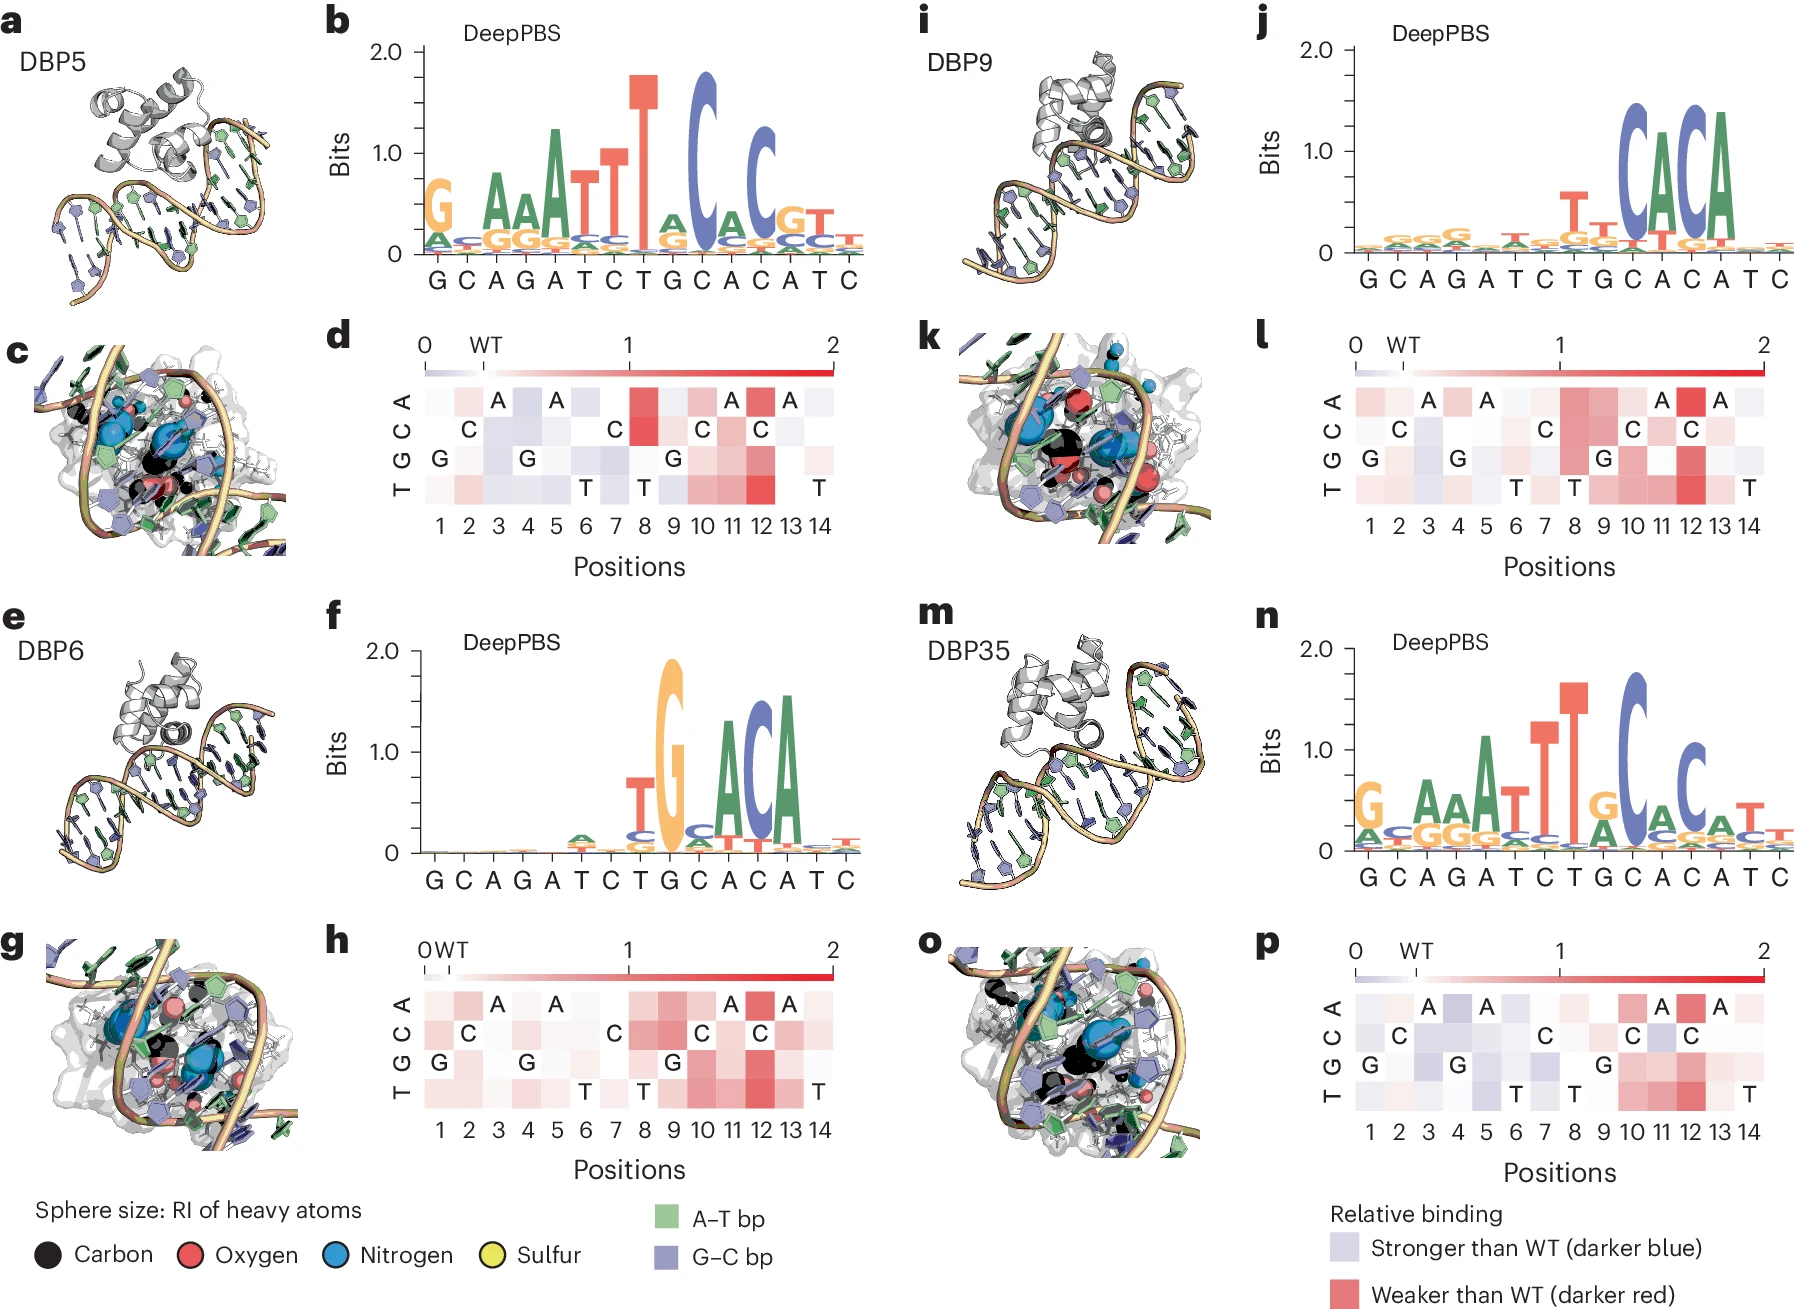
\includegraphics[width=0.8\paperwidth]{./pdnafigs/fig5.png}}
 % archetecture.png: 1149x508 px, 72dpi, 40.53x17.92 cm, bb=0 0 1149 508
        \caption[Application of DeepPBS to in silico-designed HTH scaffolds targeting a specific DNA sequence.]{\textbf{Application of DeepPBS to in silico-designed HTH scaffolds targeting a specific DNA sequence.} ({\bf a,e,i,m}) Design models of four different synthetic
HTH proteins targeting the DNA sequence GCAGATCTGCACATC (design based
on DNA sequence from PDB ID 1L3L, canonical B-DNA structure used for e and
i, co-crystal-derived DNA structure used for a and m), obtained from a recent
sequence-specific DNA binder design study 34
. ({\bf b,f,j,n}) DeepPBS ensemble
predictions based on each design model shown in a, e, i and m, respectively.
As expected, the predictions for DBP5 and DBP35 were very similar due to
comparable designs (see ‘Data availability’ section). ({\bf c,g,k,o})  DeepPBS assessment
of heavy atom level RI scores for each interface in the design models shown in
{\bf a, e, i and m} respectively. ({\bf d,h,l,p}) Relative binding activity (phycoerythrin/
fluorescein isothiocyanate normalized to the no-competitor condition) of all
possible single base-pair mutations obtained via flow cytometry analysis 34 in
yeast display competition assays for each of the four HTH proteins shown in
{\bf a, e, i and m} respectively. Blue indicates competitor mutations where
competition was stronger than with the WT competitor, while red indicates
competitor mutations where competition was weaker.}
  \label{fig:pdna5}
\end{figure}
\end{center}
